\documentclass[xcolor=table,bigger,unknownkeysallowed]{beamer}
\usetheme{SimplePlus}
\usepackage[utf8]{inputenc}
\usepackage[T1]{fontenc}
\usepackage[english]{babel}
\usepackage{fixltx2e}
\usepackage{graphicx}
\usepackage{epsfig}
\usepackage{longtable}
\usepackage{float}
\usepackage{wrapfig}
\usepackage{soul}
\usepackage{textcomp}
\usepackage{marvosym}
\usepackage{wasysym}
\usepackage{latexsym}
\usepackage{amssymb}
\usepackage{tabu}
\usepackage{tabularx}
\usepackage{booktabs}
\usepackage[margin=15pt,font={small,sf,it},labelfont=bf]{caption} 
\usepackage{hyperref}
\tolerance=1000
\providecommand{\alert}[1]{\textbf{#1}}
\usepackage{etoolbox}
\newcommand{\icon}[1]{\includegraphics[height=20pt,width=20pt]{#1}}
\usepackage{pgfplots}
\usepackage{tabu}
\usepackage{subcaption}
\usepackage{multirow}
\usepackage{pdfpages}

\usepackage{tikz}
\usetikzlibrary{matrix,positioning,fit,fadings}
\def\drowsyColor{green!80!black}       

\title{Efficient Buffer Overflow Mitigation In Virtualized Clouds Using Intel EPT-based Sub-Page Write
Protection Support}
\author{\textit{Stella Bitchebe, Scientific Days Cameroon, December 20, 2022}}
\date{~}
% More styles for bullets
\usepackage{pifont}
\usepackage{booktabs}
\usepackage[natbib=true, bibstyle=authoryear, citestyle=authoryear-comp]{biblatex}
\usepackage{beamerthemesplit}
\usetheme{progressbar}
\usecolortheme{progressbar}
%\institute{\vskip1ex Rennes - April, 29}
\definecolor{tableShade}{HTML}{787878}
\definecolor{tableShade2}{HTML}{606060}
\progressbaroptions{headline=none, frametitle=ckcompliant}
\newcommand{\myitem}{\item[\vspace{0.5ex}]}
\newcommand{\myemph}[1]{\textcolor{red}{\bf #1}}
\newcommand{\blueemph}[1]{\textcolor{blue}{\bf #1}}
\usepackage{lmodern}
\usepackage{ulem} 

% \AtBeginSection[]
% {
%   \begin{frame}<beamer>%{Outline}
% 	\thispagestyle{empty}
% 	\small \tableofcontents[currentsection,hideothersubsections]
% 	\addtocounter{framenumber}{-1}
%   \end{frame}
% }

\setbeamersize{text margin left=0em,text margin right=0em}

\usepackage{tikz,pgfplots}
\usetikzlibrary{pgfplots.groupplots}
\usepackage{pgfplotstable}
\usepgfplotslibrary{external} 
\usetikzlibrary{patterns}
\usepgfplotslibrary{fillbetween}
\usetikzlibrary{matrix,positioning,fit,fadings}
\tikzfading[name=energyPropFading,bottom color=transparent!100,top color=transparent!0]
\usepackage{color, colortbl}
\hypersetup{}

\definecolor{codegreen}{rgb}{0,0.6,0}
\definecolor{codegray}{rgb}{0.5,0.5,0.5}
\definecolor{codepurple}{rgb}{0.58,0,0.82}
\definecolor{backcolour}{rgb}{0.95,0.95,0.92}
\definecolor{americanrose}{rgb}{1.0, 0.01, 0.24}
\definecolor{airforceblue}{rgb}{0.0, 0.0, 1.0}

\newenvironment{variableblock}[3]{% 3 args
  \setbeamercolor{block body}{#2} %2nd arg
  \setbeamercolor{block title}{#3}
  \begin{block}{#1}}{\end{block}
}

\newenvironment{coloredtitleblock}[1]{% 
  \begin{block}{\textcolor{blue}{\bf #1}}}{\end{block}
}

\tikzfading[name=myfading, bottom color=transparent!100, top color=transparent!0]

\begin{document}

\frame[plain]{
\includegraphics[page=1,width=\textwidth]{title.pdf}}
%\maketitle

%%%%%%%%%%%%%%%%%%%%%%%%%%%%%%%%%%%%%%%%%%%%%%%%%%%%%%%%%%%%%%%%%%%%%%%%%%%%%%%%%%%
\section{Context: Buffer Overflow in Virtualized Clouds}
\subsection{Importance of Buffer Overflow}
\subsection{Virtualized Clouds}
%%%%%%%%%%%%%%%%%%%%%%%%%%%%%%%%%%%%%%%%%%%%%%%%%%%%%%%%%%%%%%%%%%%%%%%%%%%%%%%%%%%
\begin{frame}
	\frametitle{Context: Buffer Overflow in Virtualized Clouds}
	%\begin{block}{Why the Cloud?}
		Why the Cloud?
		\begin{itemize}
			\item Attractive costs (e.g., \textit{Faas})
			\item Management tasks simplification (e.g., \textit{SaaS, IaaS})
			\item Efficiency of Cloud computing
		\end{itemize}
	%\end{block}

	\pause
	
	%\begin{block}{Virtualized Cloud Infrastructure}	
	Virtualized Cloud Infrastructure
	\begin{figure}
	\centering
	\fcolorbox{white}{white}{
		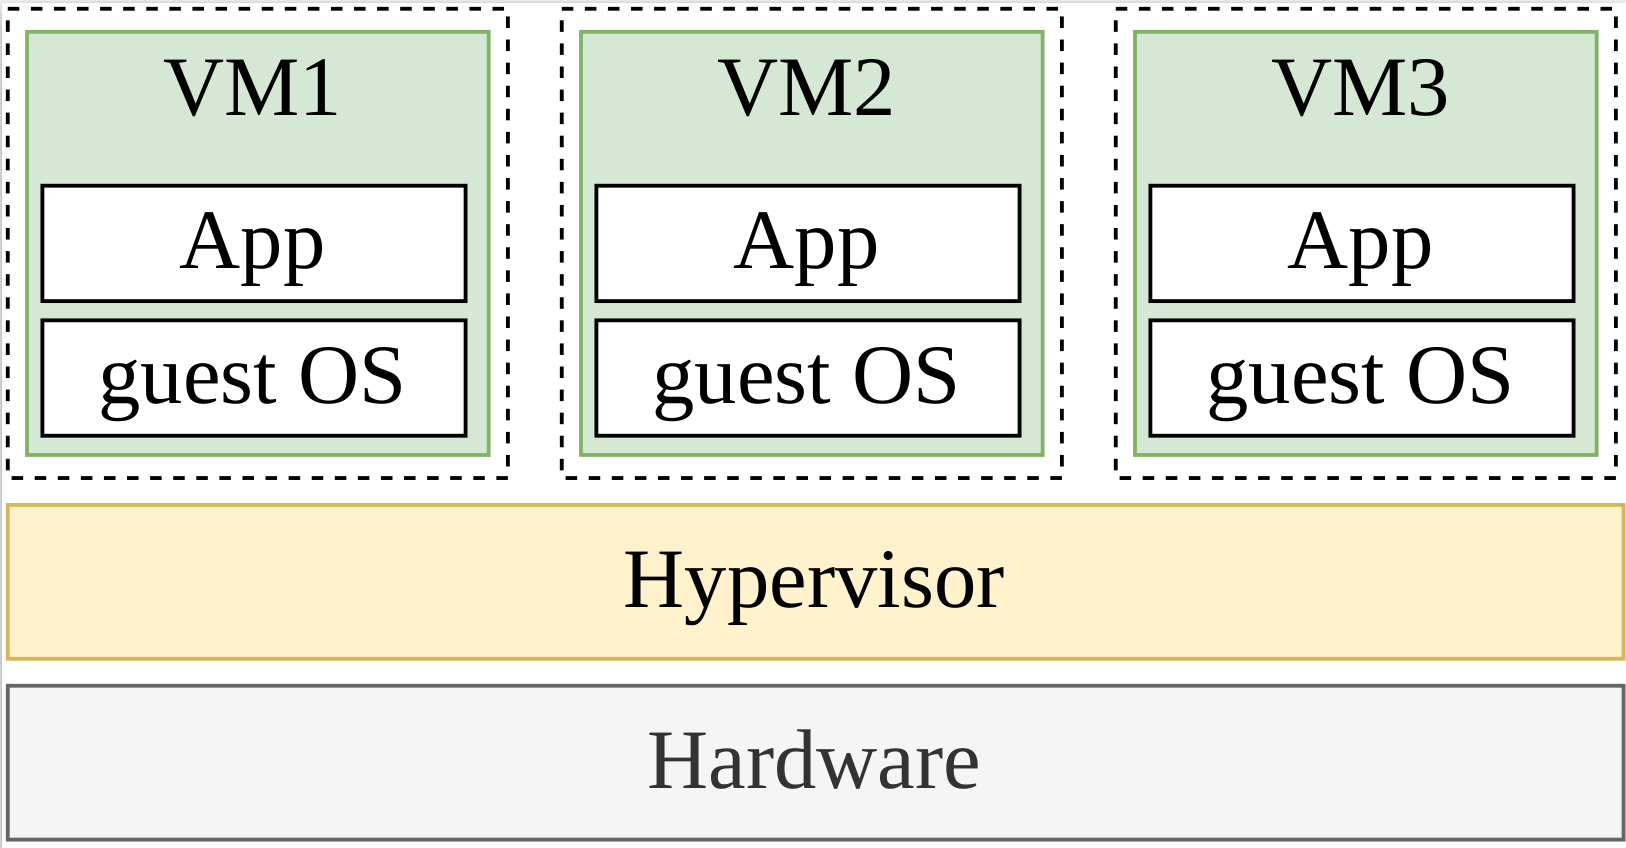
\includegraphics[width=.45\columnwidth]{fig/type1.png}
	}
	\end{figure}
	%\end{block}
\end{frame}
%---------------------------------------------
\begin{frame}
	\frametitle{Context: Buffer Overflow in Virtualized Clouds}
	What is buffer overflow?
	\begin{figure}
		%\centering
		\fcolorbox{white}{white}{
			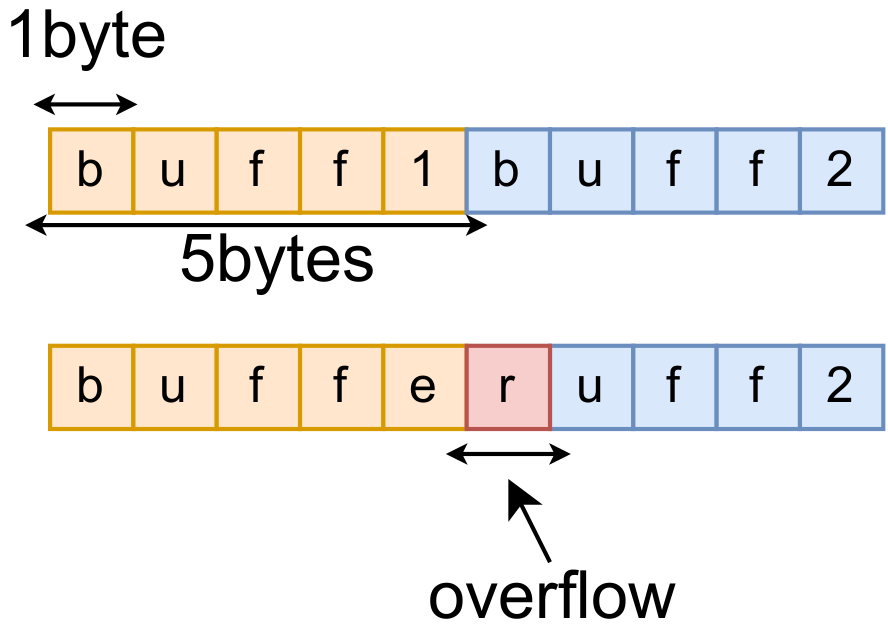
\includegraphics[width=.27\columnwidth]{fig/overflow.png}
		}
	\end{figure}

	\pause
	
	Importance of Buffer Overflow\\
	\ding{108} 70\% Google Chrome's bugs\\
	\ding{108} 70\% of Microsoft vulnerabilities\\
	\ding{108} Top vulnerability in 2022
\end{frame}
%%%%%%%%%%%%%%%%%%%%%%%%%%%%%%%%%%%%%%%%%%%%%%%%%%%%%%%%%%%%%%%%%%%%%%%%%%%%%%%%%%%
\section{State-of-the-art Techniques}
\subsection{Canary}
\subsection{Guard Page}
\subsection{Hardware Capabilities}
%%%%%%%%%%%%%%%%%%%%%%%%%%%%%%%%%%%%%%%%%%%%%%%%%%%%%%%%%%%%%%%%%%%%%%%%%%%%%%%%%%%
\begin{frame}
\frametitle{State-of-the-art Techniques} 

\begin{overprint}
	\onslide<1>	

	\begin{figure}
		\begin{subfigure}{.48\linewidth}
			\ding{108} Canary\\
			\fcolorbox{white}{white}{
				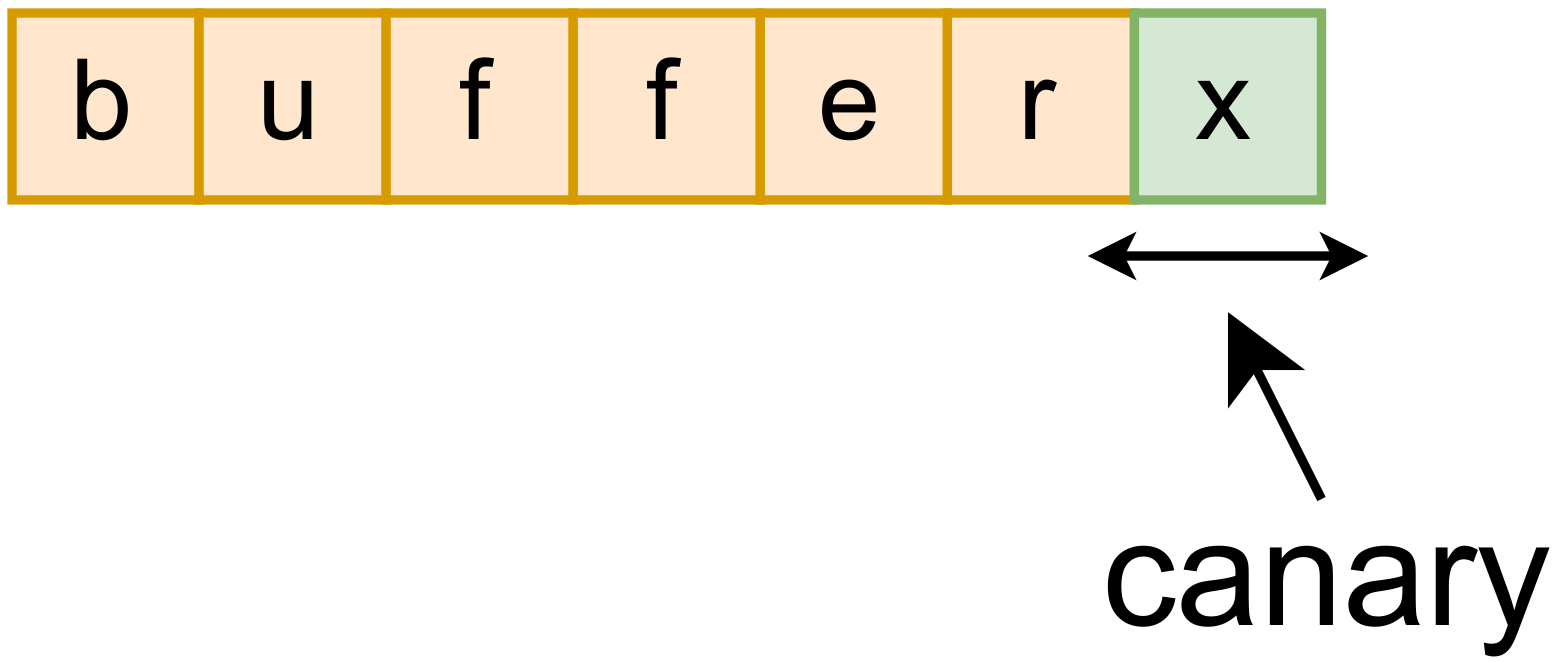
\includegraphics[width=.4\columnwidth]{fig/canary.png}
			}		
		\end{subfigure}
	\end{figure}
	
	\onslide<2>	

	\begin{figure}
		\centering
		\begin{subfigure}{.48\linewidth}
			\centering
			\ding{108} Canary\\
			\fcolorbox{white}{white}{
				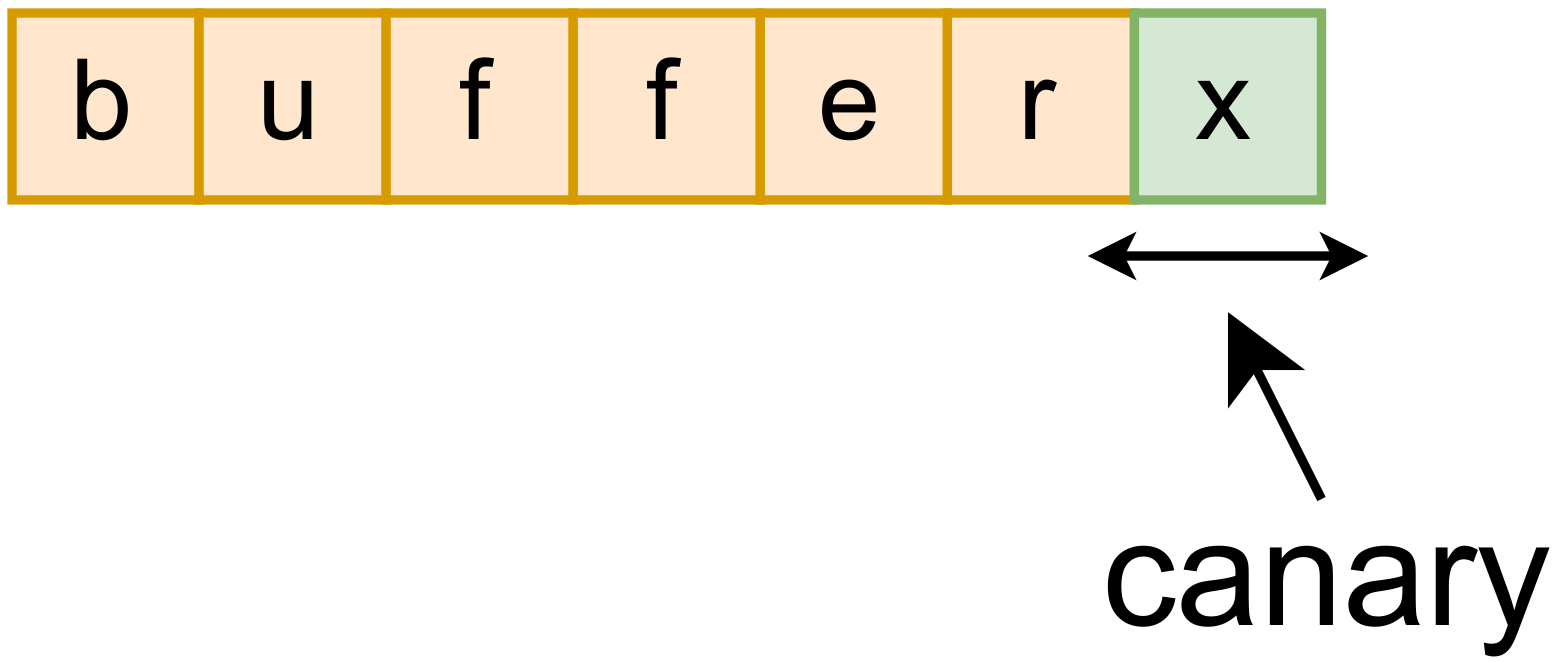
\includegraphics[width=.4\columnwidth]{fig/canary.png}
			}		
		\end{subfigure}
		\begin{subfigure}{.48\linewidth}	
			\centering
			\ding{108} Guard Page\\
			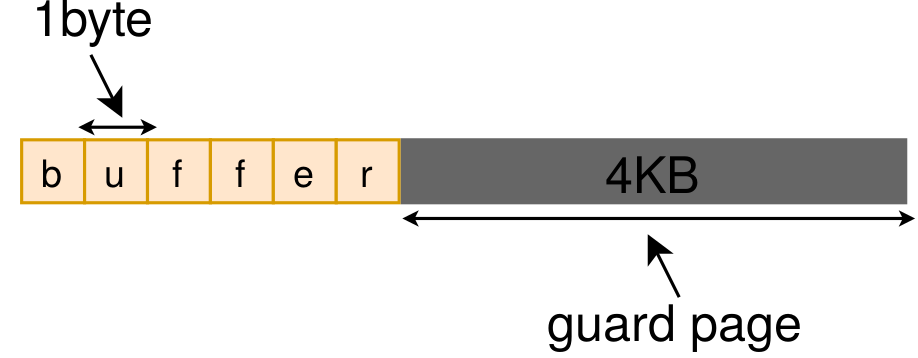
\includegraphics[width=.7\columnwidth]{fig/gp.png}
		\end{subfigure}
	\end{figure}

	\onslide<3>	

	\begin{figure}
		\centering
		\begin{subfigure}{.48\linewidth}
			\centering
			\ding{108} Canary\\
			\fcolorbox{white}{white}{
				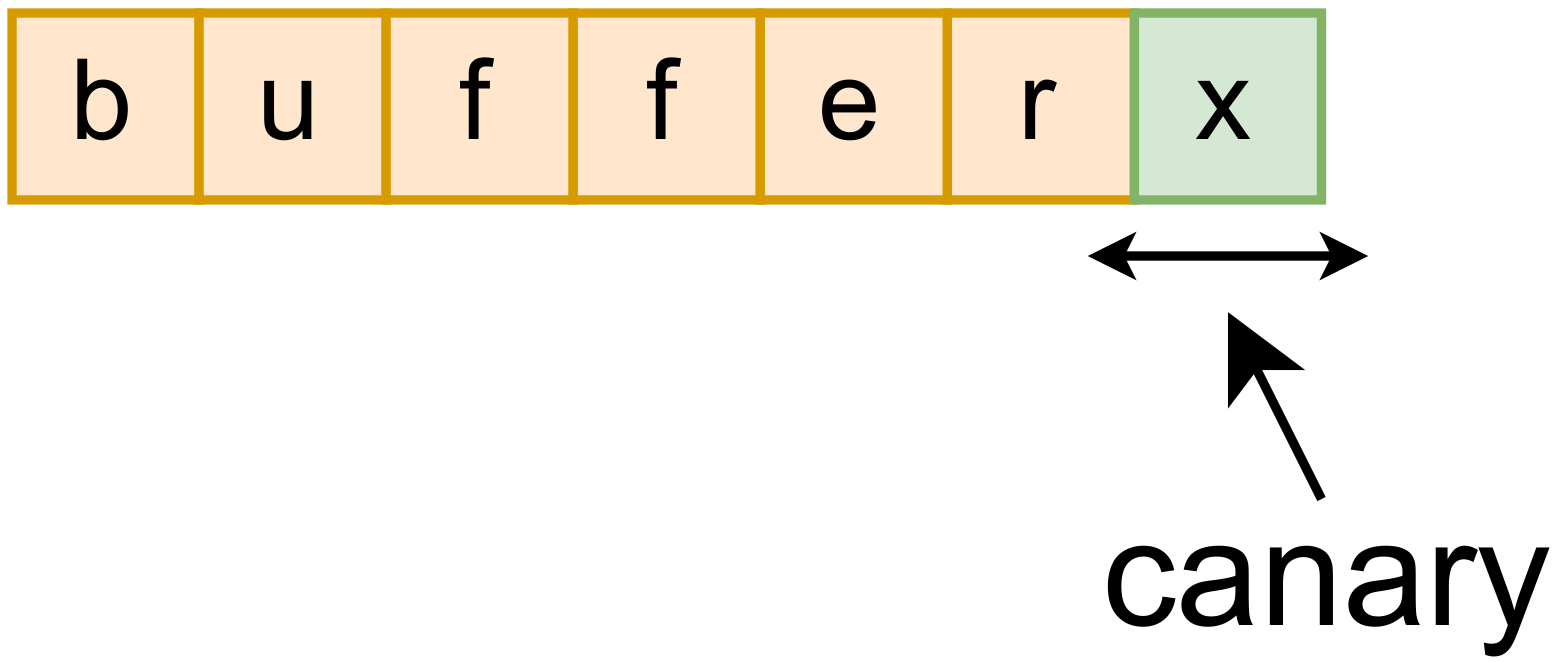
\includegraphics[width=.4\columnwidth]{fig/canary.png}
			}		
		\end{subfigure}
		\begin{subfigure}{.48\linewidth}	
			\centering
			\ding{108} Guard Page\\
			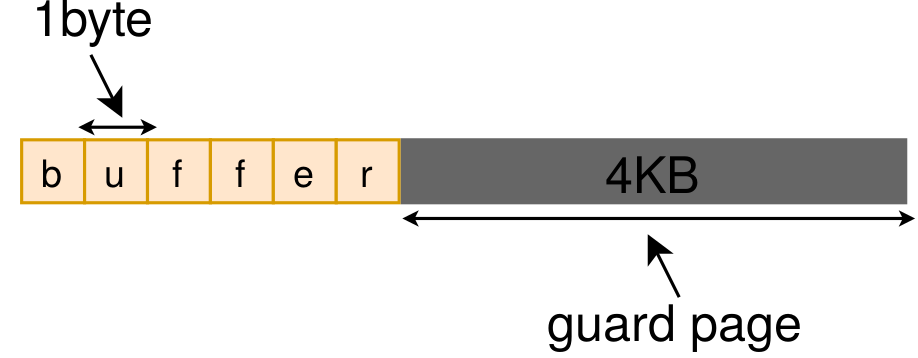
\includegraphics[width=.7\columnwidth]{fig/gp.png}
		\end{subfigure}
	\end{figure}

	\ding{108} Hardware Capabilities\\
	CHERI: Capabilities Hardware Enhance RISC-V Instructions
\end{overprint}

\end{frame}
%%%%%%%%%%%%%%%%%%%%%%%%%%%%%%%%%%%%%%%%%%%%%%%%%%%%%%%%%%%%%%%%%%%%%%%%%%%%%%%%%%%
\section{Secure Allocators: SlimGuard}
%%%%%%%%%%%%%%%%%%%%%%%%%%%%%%%%%%%%%%%%%%%%%%%%%%%%%%%%%%%%%%%%%%%%%%%%%%%%%%%%%%%
\begin{frame}
	\frametitle{Secure Allocators: SlimGuard} 
	\textbf{Overview}\\
	\vspace*{.5cm}
	\ding{108} State-of-the-art BIBOP (Big Bag Of Pages) secure allocator\\
	\ding{108} Published in 2019\\
	\ding{108} Has proven more memory-efficient than other state-of-the-art BIBOP allocators (Guarder, FreeGuard, etc.)\\
	\ding{108} Available and functional code\\
	\pause
	\ding{108} Fine-grained bag sizes (not size-of-two -2, 8, 16, ...- like others)
	\vspace*{-.3cm}
	\begin{figure}
		\centering
		\fcolorbox{white}{white}{
			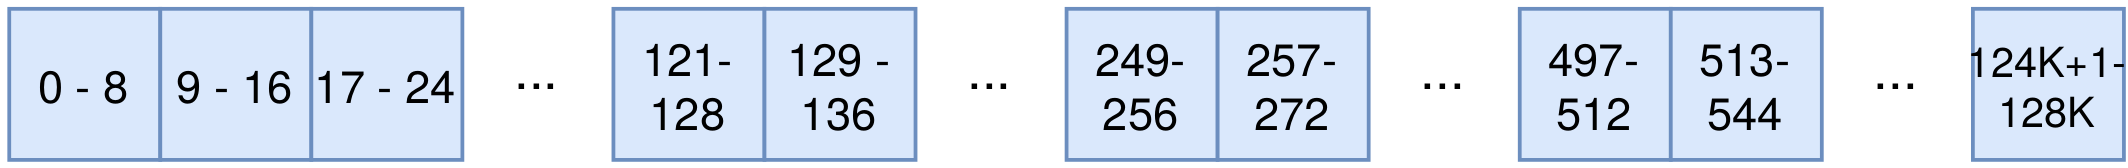
\includegraphics[width=.5\columnwidth]{fig/slim_classes.png}
		}		
	\end{figure} 
	\pause
	\blueemph{Protection policy: applied at the bag scale}\\ 
	- Configurable proportion of guard pages P\\
	- 1/P allocation pages between 2 guard pages		
\end{frame}
%---------------------------------------------
\begin{frame}
	\frametitle{Secure Allocators: SlimGuard}  
	\textbf{Limits}\\
	\vspace*{.5cm}
	\begin{figure}
		\centering
		\begin{subfigure}{.48\linewidth}
			\centering
			Significant memory overhead\\
			\fcolorbox{white}{white}{
				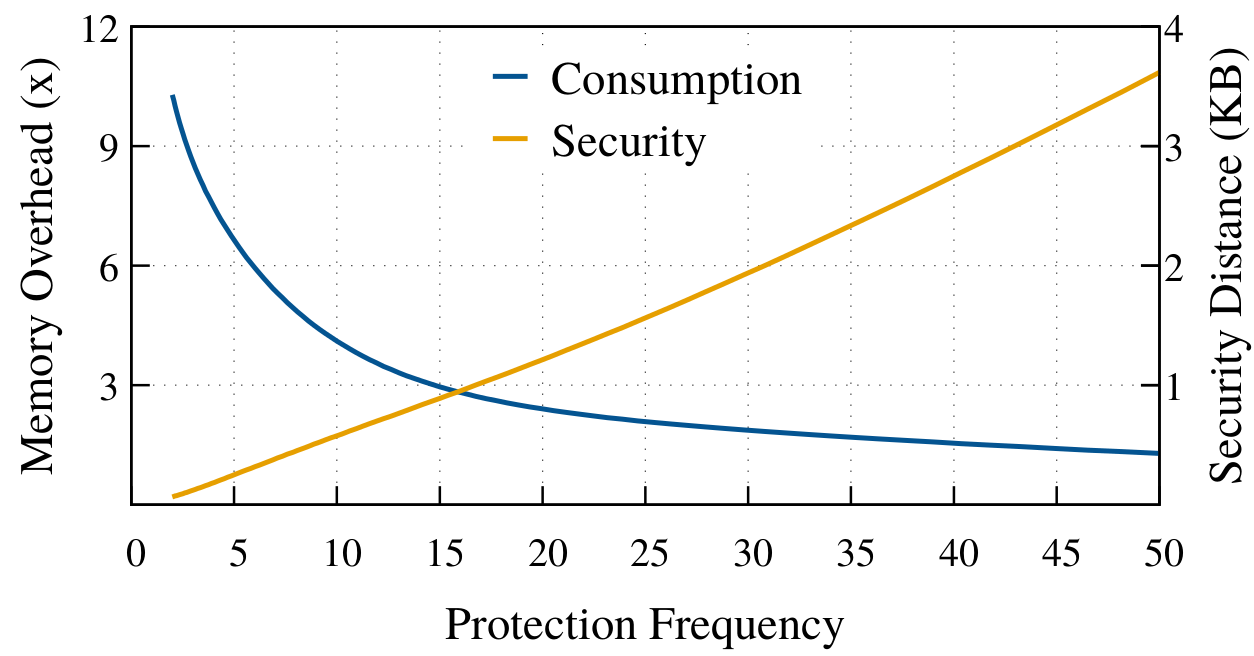
\includegraphics[width=.8\columnwidth]{fig/slim_limit1.png}
			}		
		\end{subfigure}
		\pause
		\begin{subfigure}{.48\linewidth}	
			\centering
			Inefficient protection policy\\
			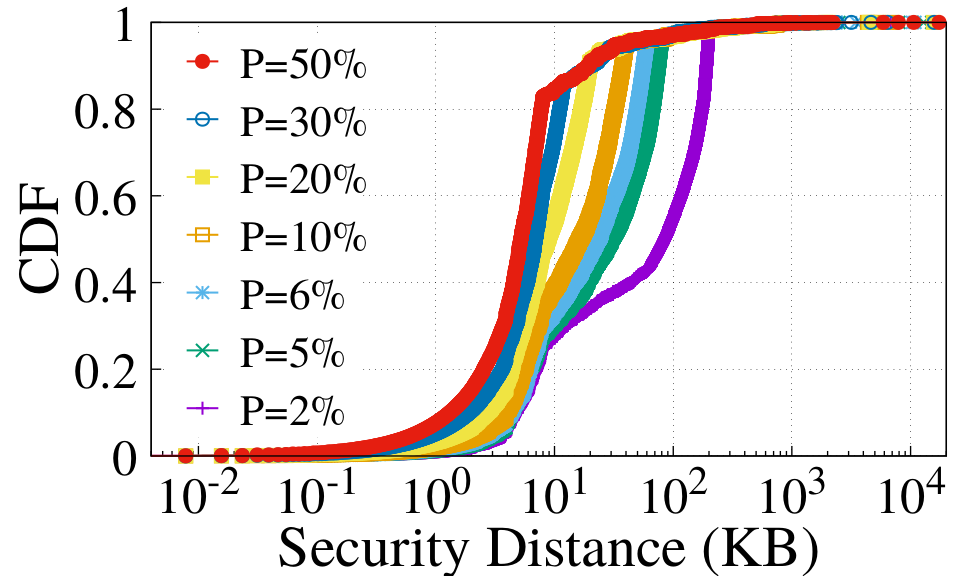
\includegraphics[width=.8\columnwidth]{fig/slim_limit2.png}
		\end{subfigure}
	\end{figure}
\end{frame}
%---------------------------------------------
\begin{frame}
	\frametitle{Secure Allocators: SlimGuard} 
	\begin{block}{Custom Protection Policy}
		\begin{figure}	
			\centering
			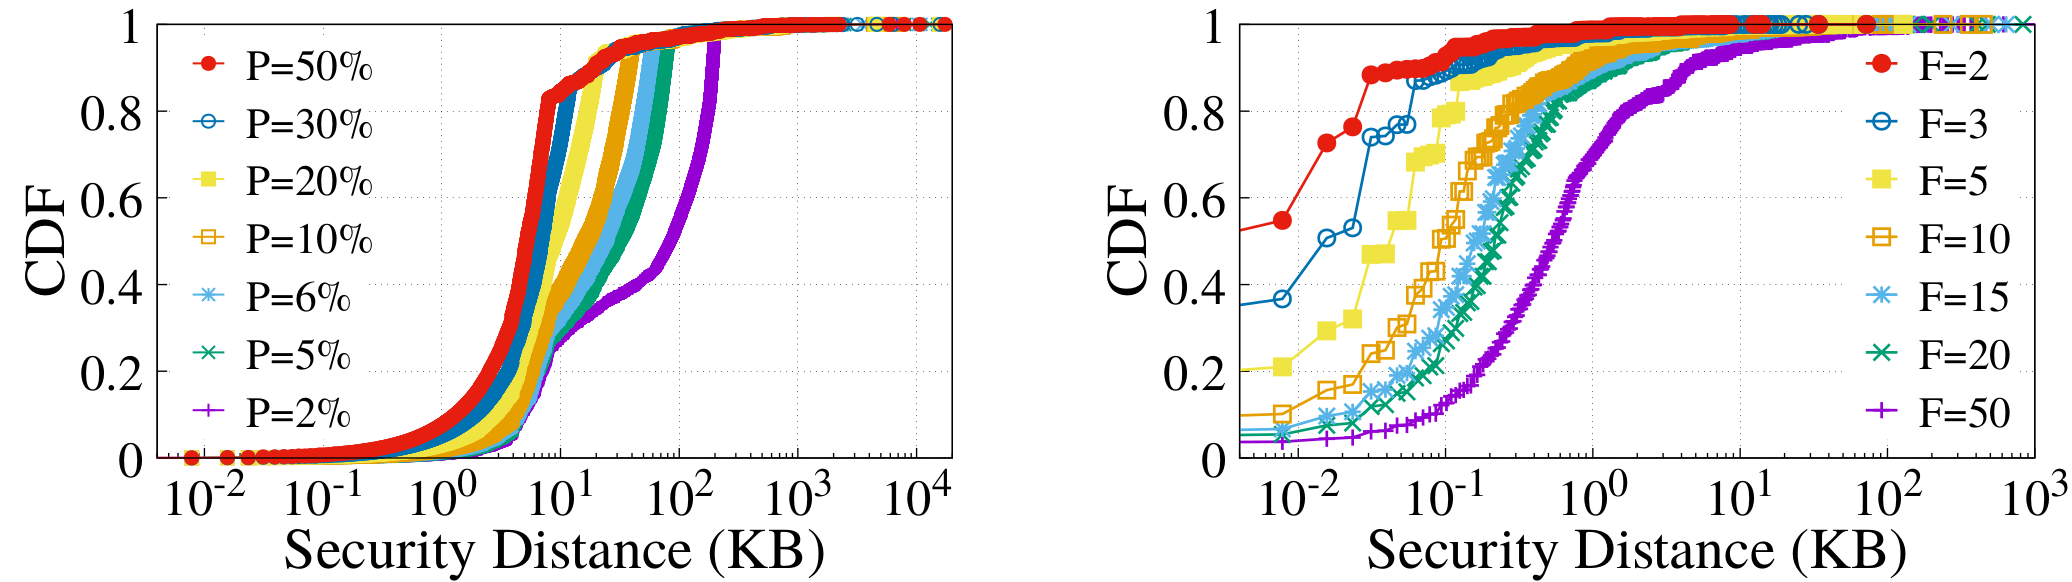
\includegraphics[width=.7\columnwidth]{fig/policy_guan.png}
		\end{figure}
	\end{block}	
	\pause
	\begin{figure}	
		\centering
		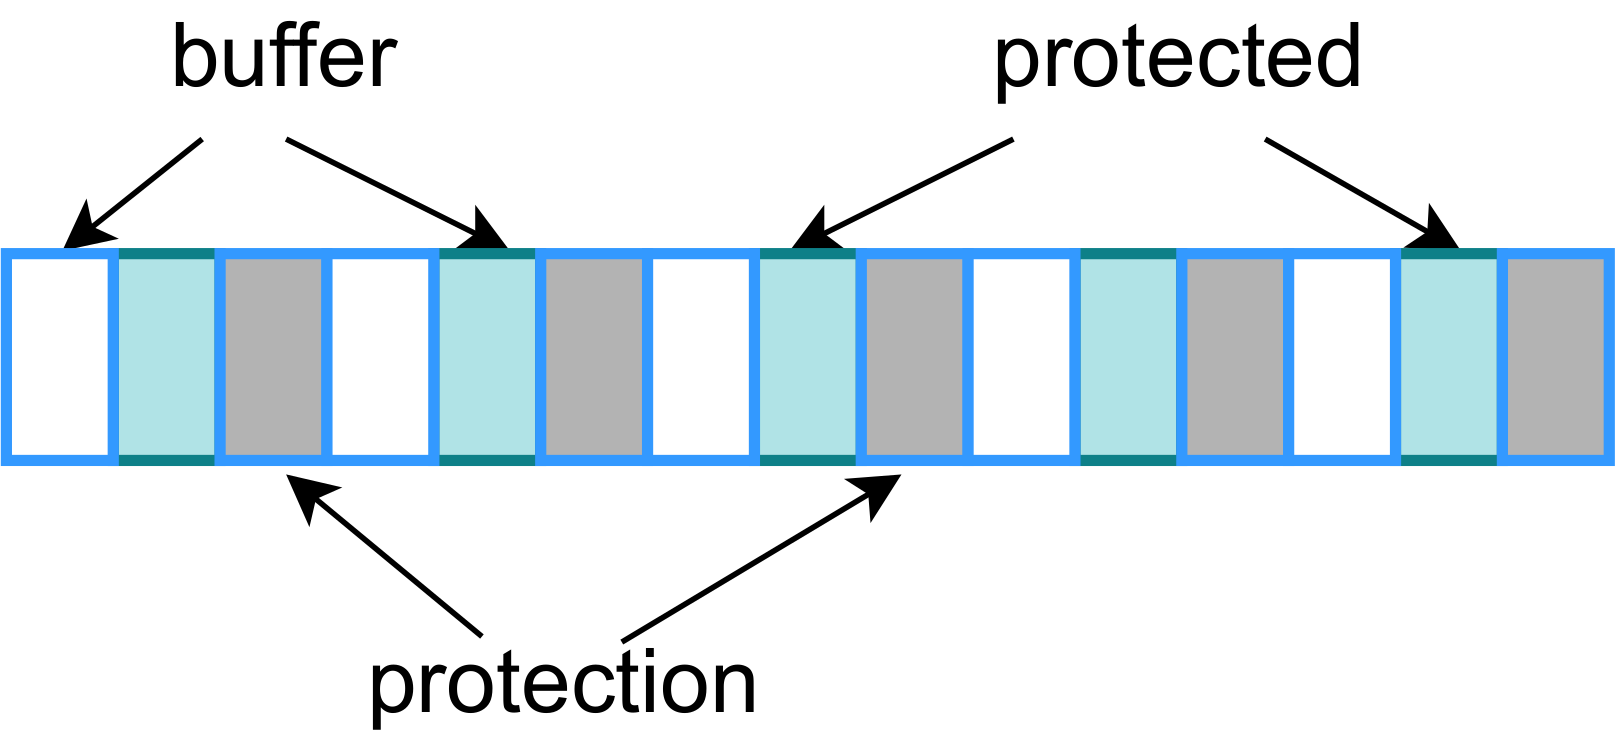
\includegraphics[width=.3\columnwidth]{fig/policy_illustration.png}
	\end{figure}
\end{frame}
%%%%%%%%%%%%%%%%%%%%%%%%%%%%%%%%%%%%%%%%%%%%%%%%%%%%%%%%%%%%%%%%%%%%%%%%%%%%%%%%%%%
\section{Problem: Dilemma between Synchronous Detection vs Memory Overhead}
%%%%%%%%%%%%%%%%%%%%%%%%%%%%%%%%%%%%%%%%%%%%%%%%%%%%%%%%%%%%%%%%%%%%%%%%%%%%%%%%%%%
\begin{frame}
	\frametitle{Synchronous Detection vs Memory Overhead} 
	\begin{overprint}
		\onslide<1>	
		Canary: \myemph{modest memory overhead} + asynchronous overflow detection\\
		Guard page: significant memory consumption + \myemph{synchronous overflow detection}
		\begin{figure}
			\centering
			\fcolorbox{white}{white}{
				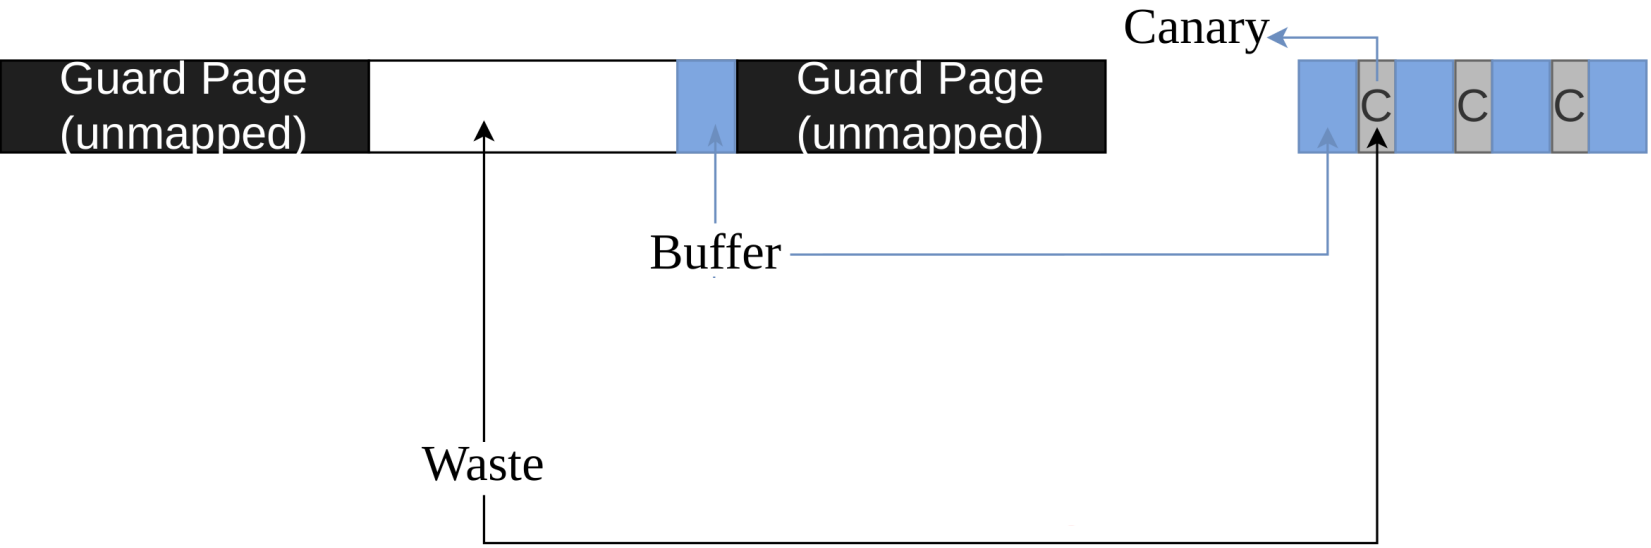
\includegraphics[width=.5\columnwidth]{fig/dilemma1.png}
			}		
		\end{figure}

		\onslide<2>	 
		\textcolor{gray}{Canary: modest memory overhead + asynchronous overflow detection}\\
		\textcolor{gray}{Guard page: significant memory consumption + synchronous overflow detection}\\
		GuaNary: \myemph{modest memory overhead + synchronous overflow detection}
		\begin{figure}
			\centering
			\fcolorbox{white}{white}{
				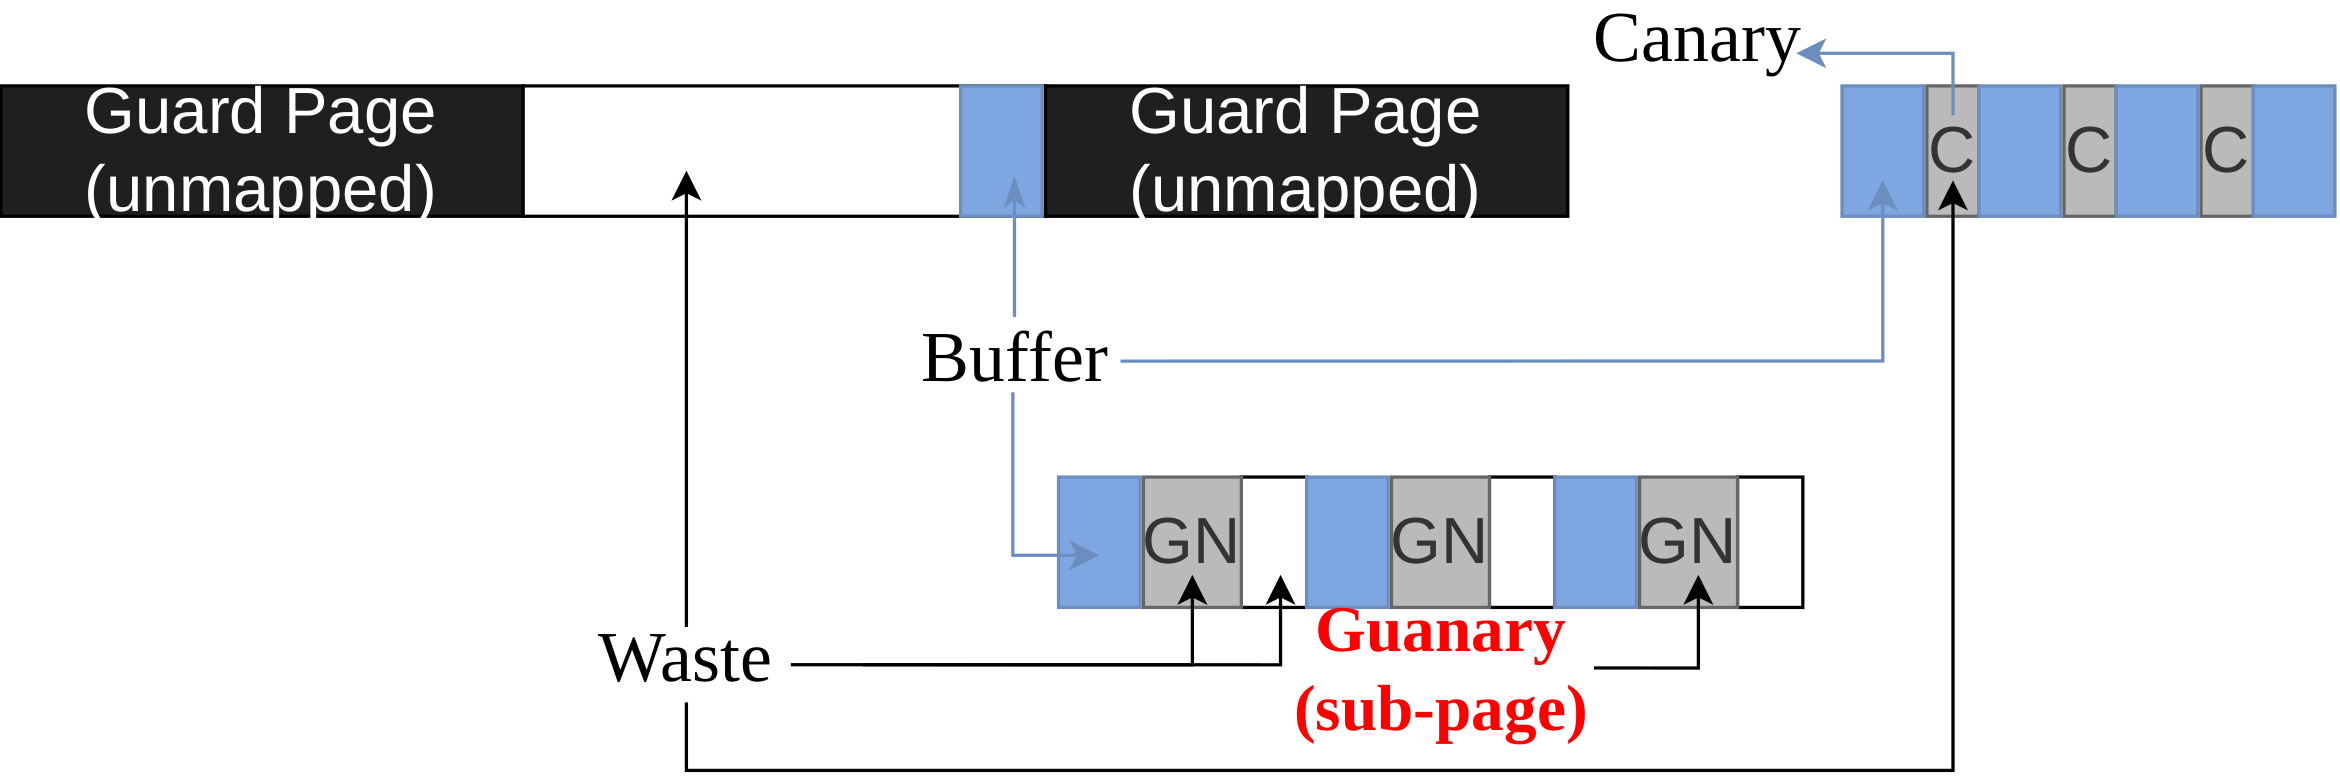
\includegraphics[width=.5\columnwidth]{fig/dilemma.png}
			}
		\end{figure}
	\end{overprint}
	
\end{frame}
%%%%%%%%%%%%%%%%%%%%%%%%%%%%%%%%%%%%%%%%%%%%%%%%%%%%%%%%%%%%%%%%%%%%%%%%%%%%%%%%%%%
\section{GuaNary: Canary and Guard Page Countermeasure}
\subsection{Intel Sub-Page write Permission (SPP)}
\subsection{Challenges}
%%%%%%%%%%%%%%%%%%%%%%%%%%%%%%%%%%%%%%%%%%%%%%%%%%%%%%%%%%%%%%%%%%%%%%%%%%%%%%%%%%%
\begin{frame}
	\frametitle{GuaNary: Canary and Guard Page Countermeasure}
	Intel Sub-Page write Permission (SPP)
	\begin{figure}
		\centering
		\fcolorbox{white}{white}{
			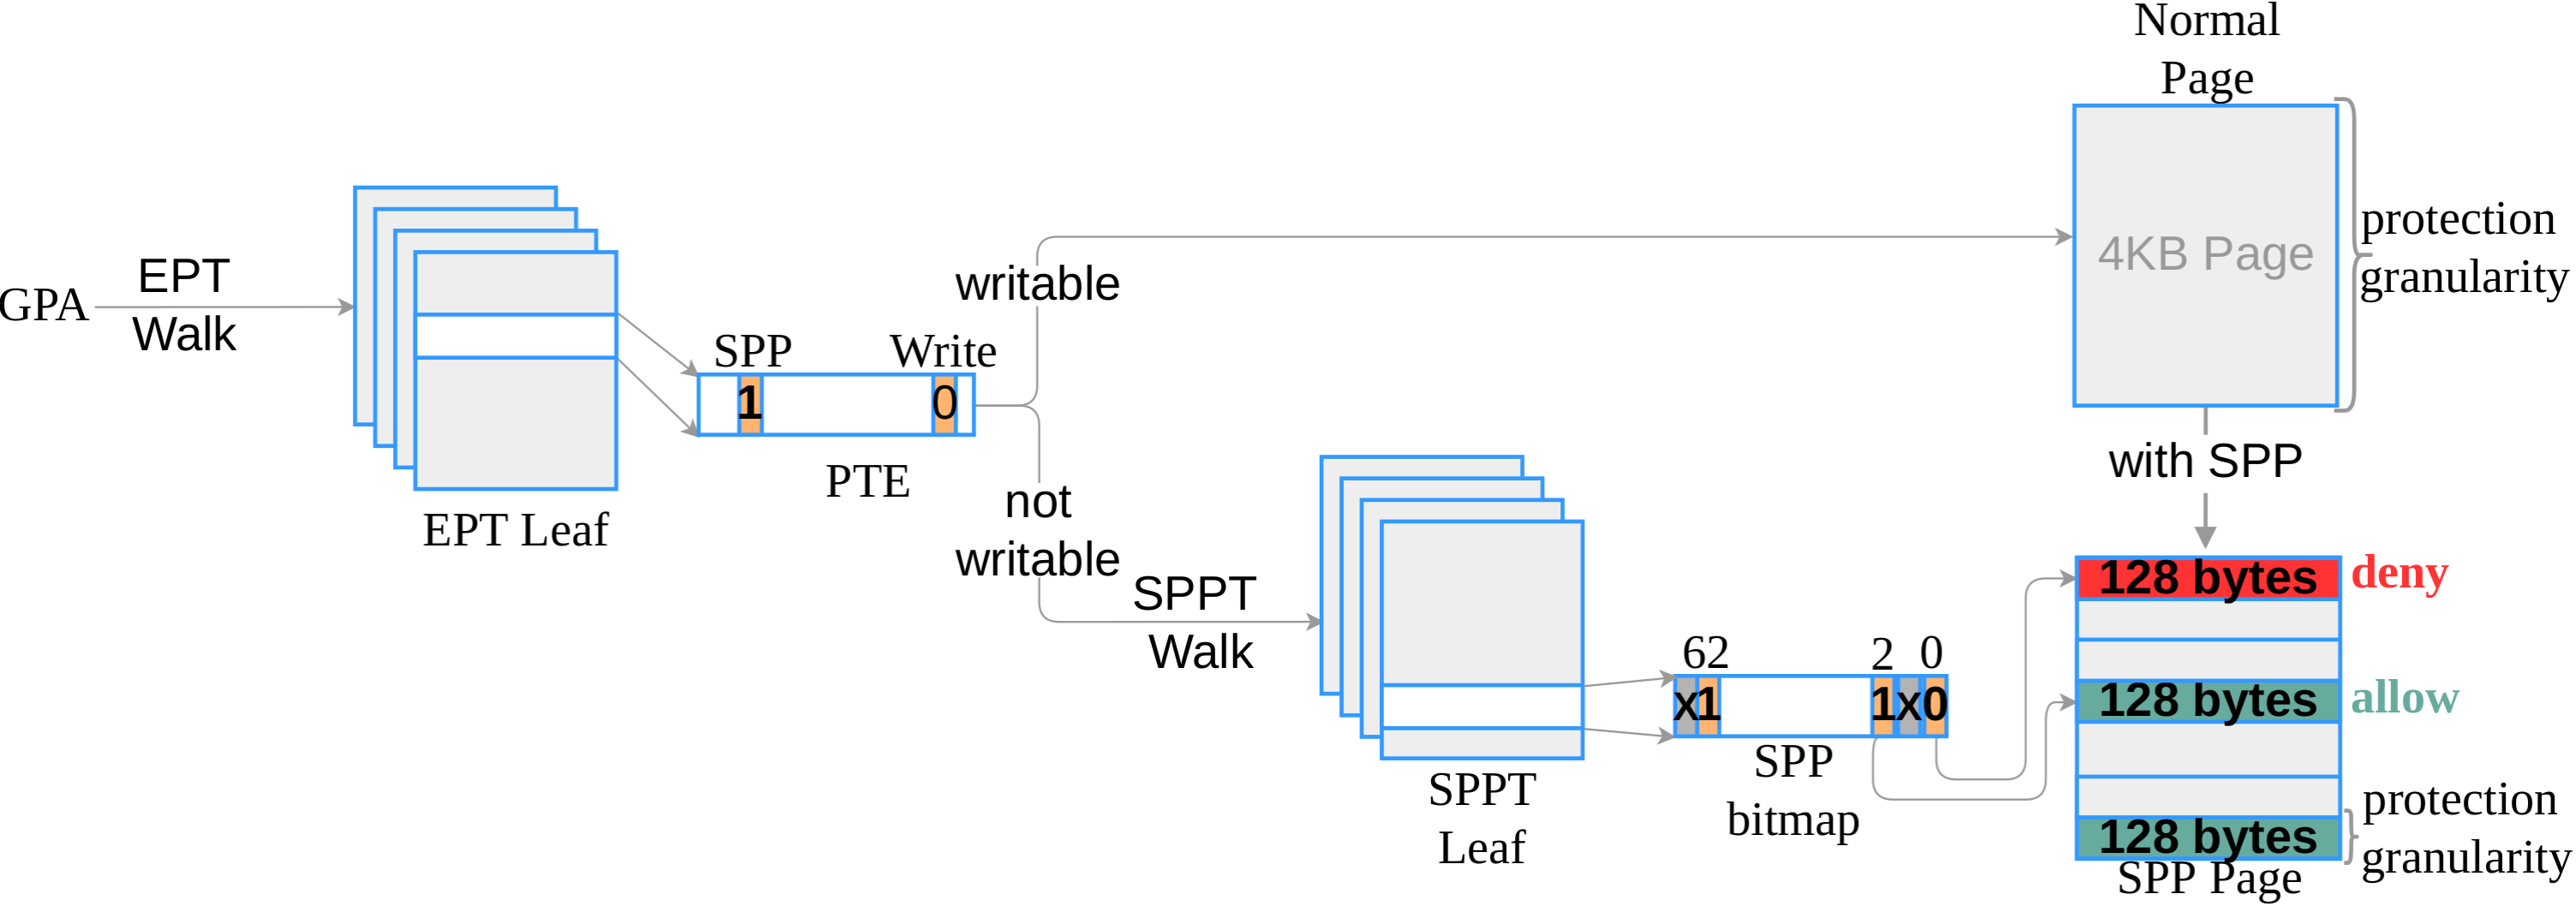
\includegraphics[width=.6\columnwidth]{fig/spp.png}
		}
	\end{figure}
\end{frame}
%---------------------------------------------
\begin{frame}
	\frametitle{GuaNary: Challenges}
	\myemph{$C_1$: One size does not fit all}
	\begin{figure}
		\centering
		\fcolorbox{white}{white}{
			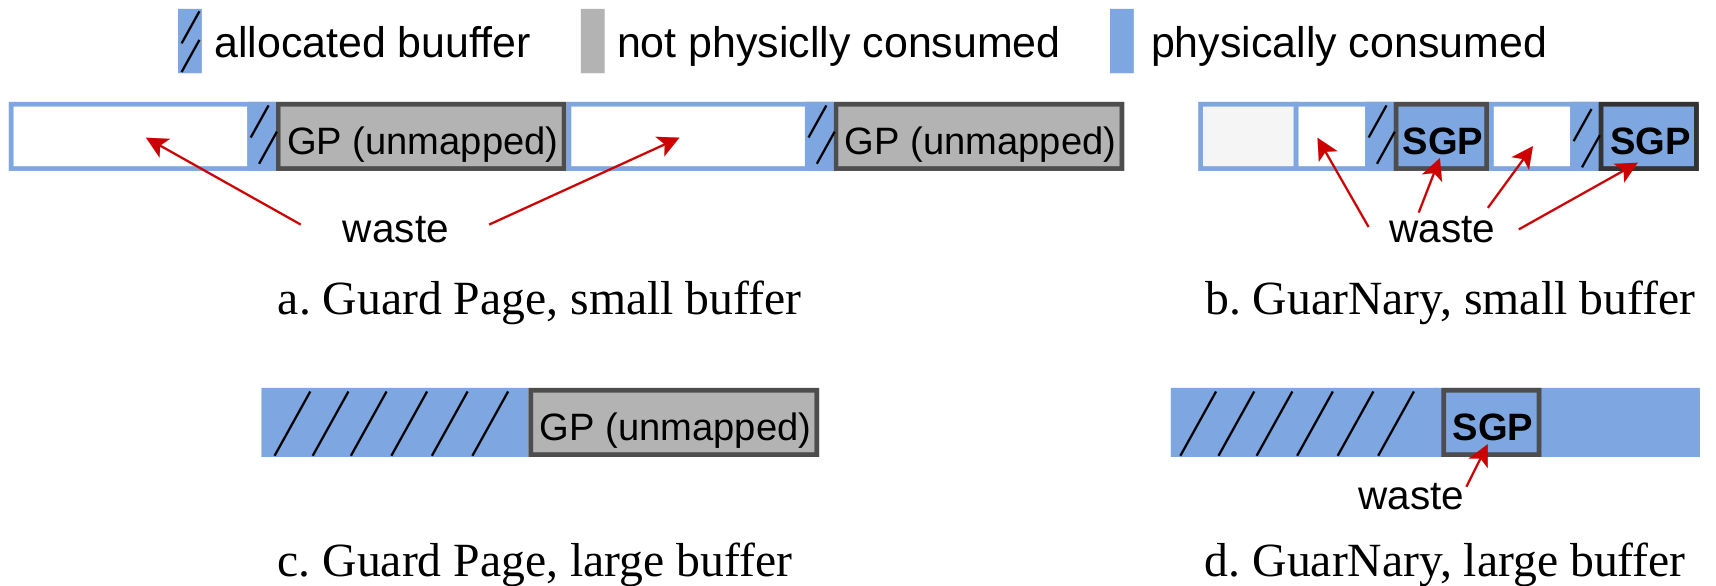
\includegraphics[width=.45\columnwidth]{fig/challenge1.png}
		}
	\end{figure}	
	\pause
	\myemph{$C_2$: Costly hypercalls}\\	
	\pause
	\myemph{$C_3$: Page heterogeneity}\\	
	\pause
	\myemph{$C_4$: SPP Page heterogeneity}
	\begin{figure}
		\centering
		\begin{subfigure}{.48\linewidth}
			\centering
			\fcolorbox{white}{white}{
				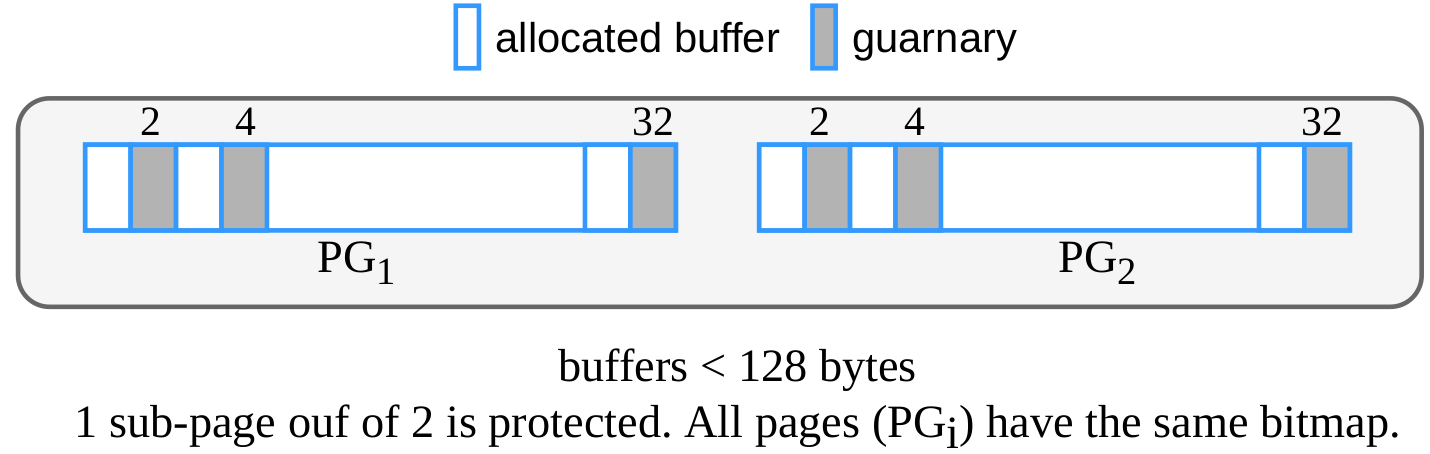
\includegraphics[width=.8\columnwidth]{fig/challenge4_1.png}
			}		
		\end{subfigure}
		\pause
		\begin{subfigure}{.48\linewidth}	
			\centering
			\fcolorbox{white}{white}{
				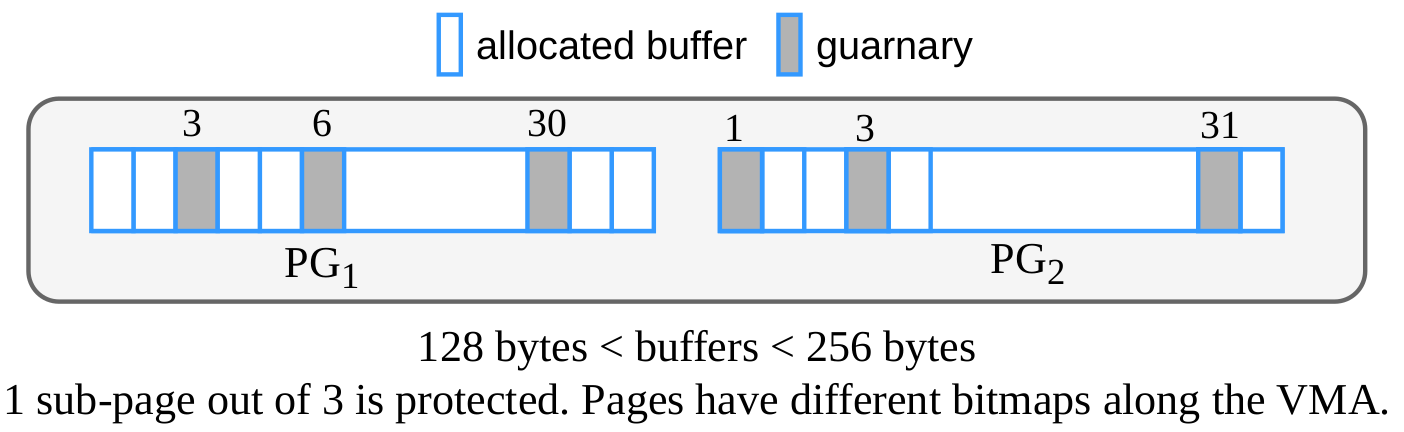
\includegraphics[width=.8\columnwidth]{fig/challenge4_2.png}
			}
		\end{subfigure}
	\end{figure}
\end{frame}

%%%%%%%%%%%%%%%%%%%%%%%%%%%%%%%%%%%%%%%%%%%%%%%%%%%%%%%%%%%%%%%%%%%%%%%%%%%%%%%%%%%
\section{LeanGuard: GuaNary-based Secure Allocator}
\subsection{Overview}
\subsection{Implementation}
%%%%%%%%%%%%%%%%%%%%%%%%%%%%%%%%%%%%%%%%%%%%%%%%%%%%%%%%%%%%%%%%%%%%%%%%%%%%%%%%%%%
\begin{frame}
	\frametitle{LeanGuard: GuaNary-based Secure Allocator} 
	\textbf{Overview}\\
	\vspace*{.5cm}
	\begin{minipage}{.48\linewidth}
		\begin{figure}
			\centering
			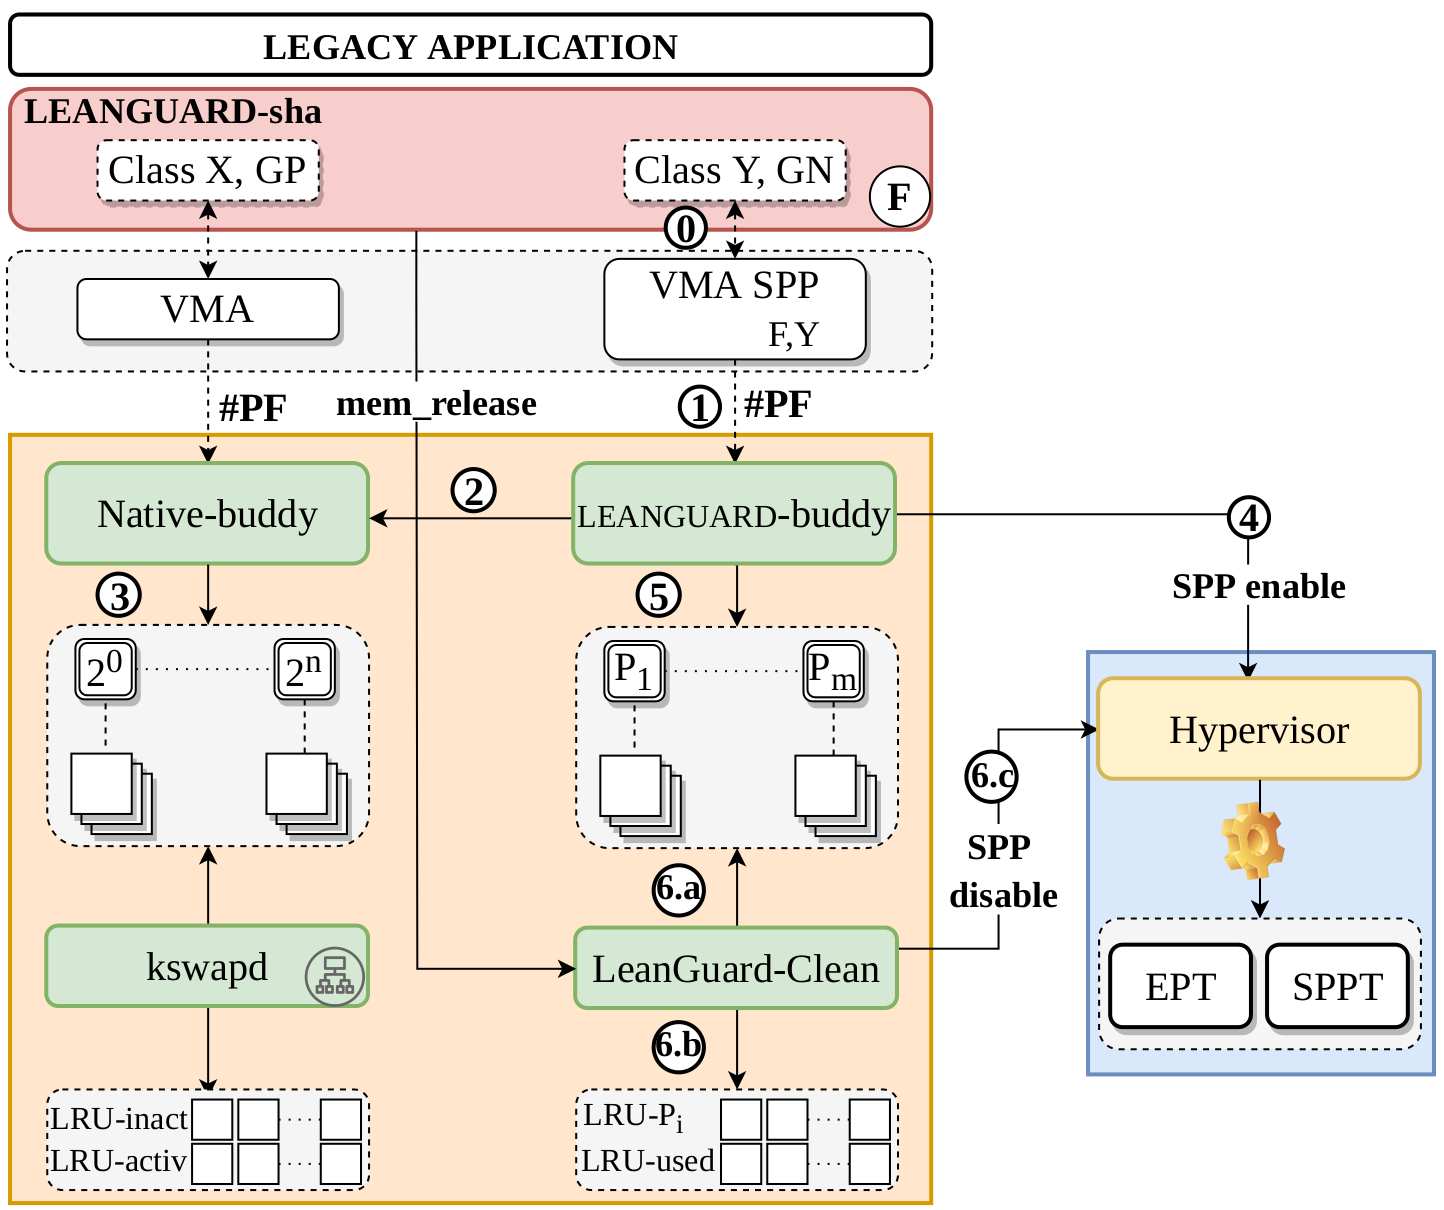
\includegraphics[width=.9\columnwidth]{fig/leanguard.png}
		\end{figure}			
	\end{minipage}
	\begin{minipage}{.48\linewidth}
		$c_1$: use GuaNary or guard page according to the size of buffers\\
		\pause
		$c_2$: batching	hypercalls for optimal performance\\
		$c_3$: new buddy allocator (LeanGuard-buddy)\\
		\pause
		$c_4$: formula to determine which pattern to use; 202 pools, one per pattern
	\end{minipage}	
\end{frame}               
%---------------------------------------------
\begin{frame}
	\frametitle{LeanGuard: GuaNary-based Secure Allocator} 
	\textbf{Implementation}\\
	\vspace*{.5cm}
	\begin{itemize}
		\item Xen hypervisor version 4.10: 600LOCs addition
		\pause
		\item Linux OS version 5.11.14: 750LOCs addition
		\pause
		\item SlimGuard secure allocator: 100LOCs addition
	\end{itemize}
\end{frame}
%%%%%%%%%%%%%%%%%%%%%%%%%%%%%%%%%%%%%%%%%%%%%%%%%%%%%%%%%%%%%%%%%%%%%%%%%%%%%%%%%%%   
\section{Evaluatons}
\subsection{Benchmarks}
\subsection{Memory Consumption}
\subsection{Performance Overhead}
%%%%%%%%%%%%%%%%%%%%%%%%%%%%%%%%%%%%%%%%%%%%%%%%%%%%%%%%%%%%%%%%%%%%%%%%%%%%%%%%%%%
\begin{frame}
	\frametitle{Evaluations} 
	\textbf{Benchmarks}\\
	\vspace*{.5cm}
	\begin{itemize}
		\item Micro-benchmark: 1GB working set application, random buffers allocation from all SlimGuard Classes
		\item Macro-benchmark: PARSEC suite
	\end{itemize}
\end{frame}
%---------------------------------------------
\begin{frame}
	\frametitle{Evaluations} 
	\textbf{Memory Consumption Results}\\
	\vspace*{-.1cm}
	\begin{figure}
		\centering
		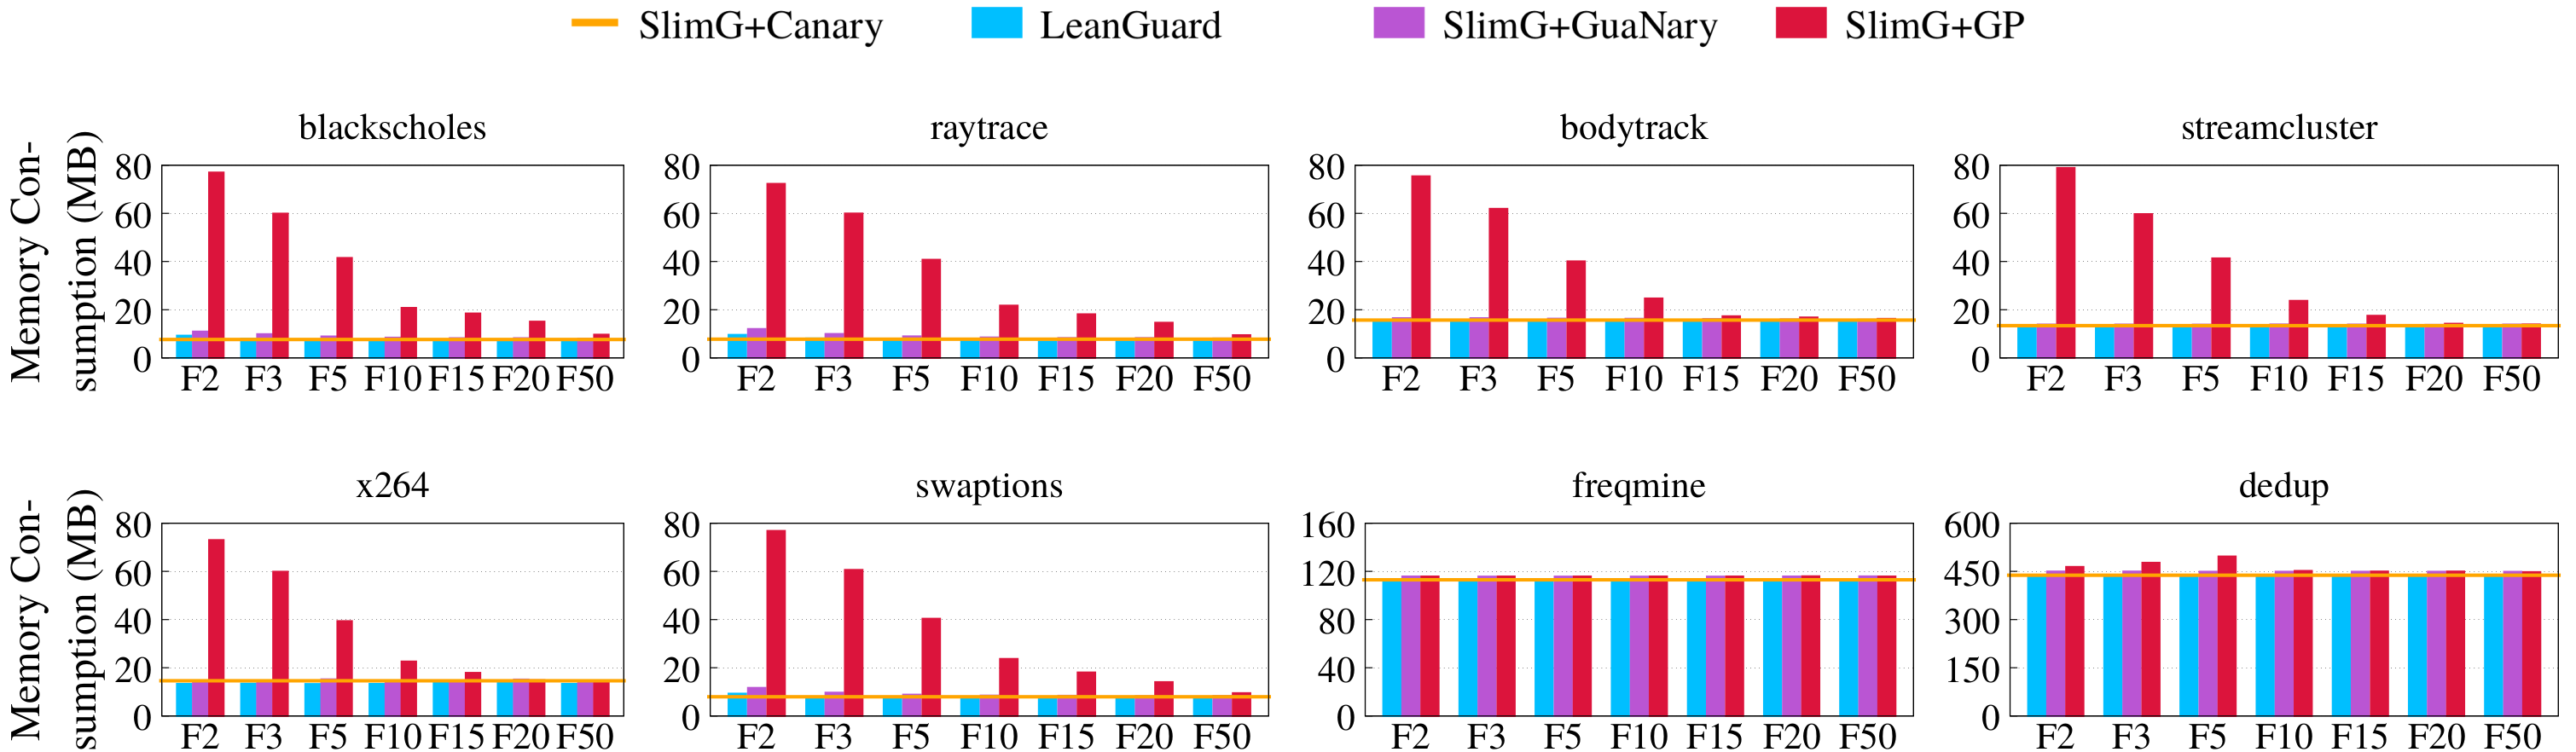
\includegraphics[width=.8\columnwidth]{fig/memory_conso.png}
	\end{figure}
	\vspace*{-.1cm}
	\begin{itemize}
		\item GuaNary effectively reduces memory consumption compared to Canary and guard page
		\item To protect \myemph{50\%} of the allocated buffers (F=2), LeanGuard on average uses \myemph{60\%} less memory compared to SlimG+GP
		\item Using the same amount of memory as SlimG+GP, LeanGuard allows protecting \myemph{25$\times$} more buffers than SlimG+GP
	\end{itemize}	
\end{frame}
%---------------------------------------------
\begin{frame}
	\frametitle{Evaluations} 
	\textbf{Performance Overhead}\\
	\begin{figure}
		\centering
		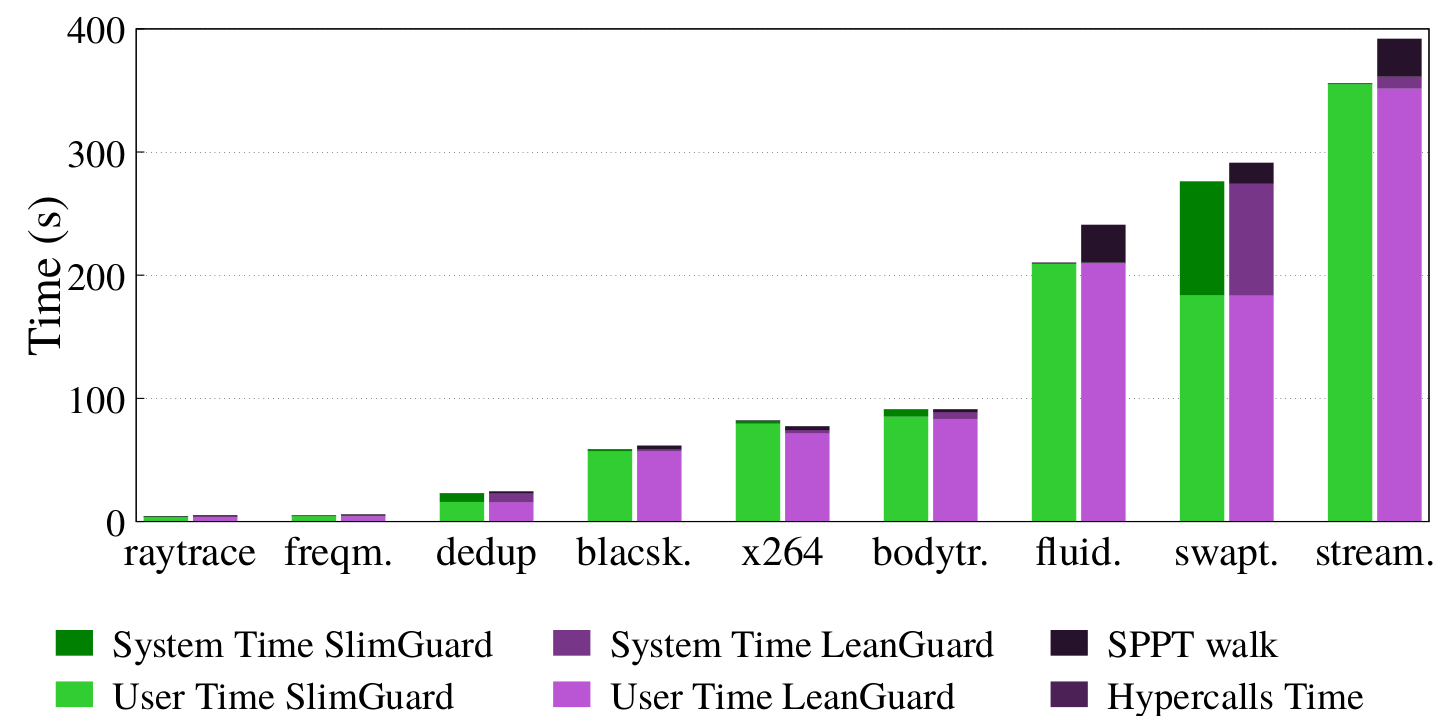
\includegraphics[width=.5\columnwidth]{fig/perf_overhead.png}
	\end{figure}	
	\begin{itemize}
		\item $\sim$7.7\% overhead on average
		\item The main source of this overhead is the SPP page table walk on TLB miss
	\end{itemize}
\end{frame}
%---------------------------------------------
\begin{frame}
	\frametitle{Evaluations} 
	\textbf{Scalability}\\
	\begin{figure}
		\centering
		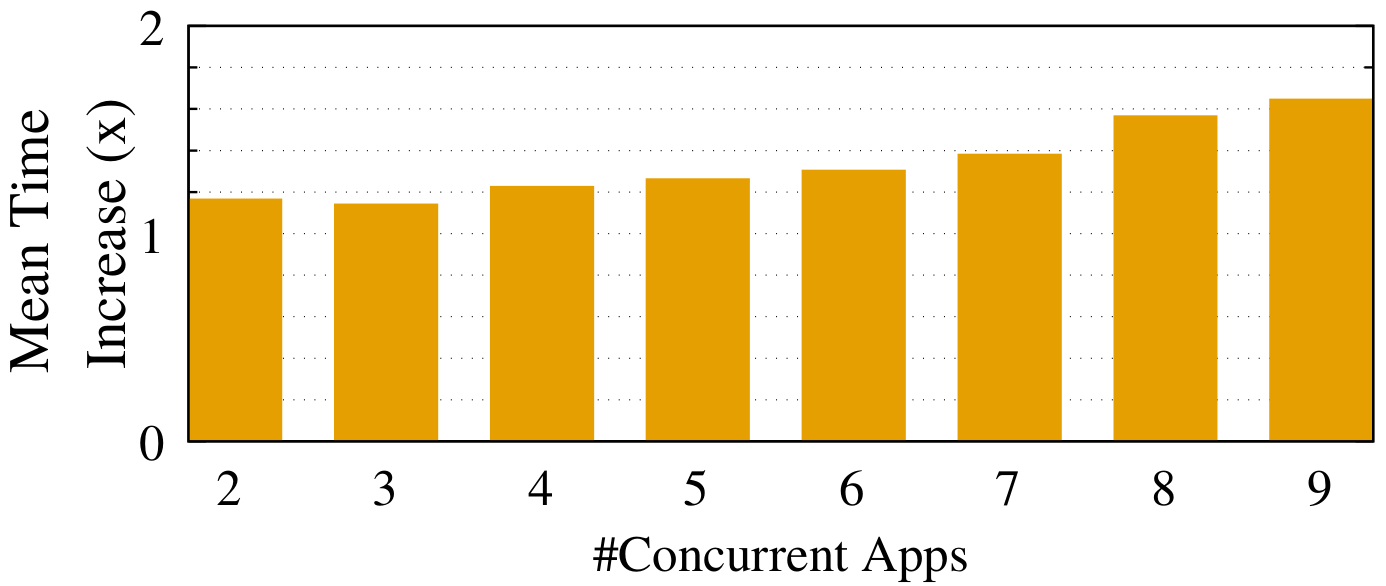
\includegraphics[width=.5\columnwidth]{fig/concurrency.png}
	\end{figure}	
	\begin{itemize}
		\item LeanGuard-buddy uses a lock mechanism
	\end{itemize}
\end{frame}
%%%%%%%%%%%%%%%%%%%%%%%%%%%%%%%%%%%%%%%%%%%%%%%%%%%%%%%%%%%%%%%%%%%%%%%%%%%%%%%%%%%   
\section{Conclusion}
%%%%%%%%%%%%%%%%%%%%%%%%%%%%%%%%%%%%%%%%%%%%%%%%%%%%%%%%%%%%%%%%%%%%%%%%%%%%%%%%%%%
\begin{frame}
\thispagestyle{empty}
\frametitle{Conclusion}	
	\begin{itemize}
		\item We introduce a novel technique to mitigate buffer overflow in virtualized clouds: \myemph{GuaNary}
		\begin{itemize}
			\item based on Intel sub-page write permission (SPP)
			\item \myemph{modest memory overhead + synchronous overflow detection}
		\end{itemize}
		\item We propose
		\begin{itemize}
			\item LeanGuard: a complete software stack that uses GuaNary
			\item LeanGuard-secure allocator: 
			\begin{itemize}
				\item consumes \myemph{8.3$\times$} less memory compared to the SlimGuard allocator (up-to-date state-of-the-art)
				\item Allows protecting \myemph{25$\times$} more buffers than SlimGuard for the same amount of memory
			\end{itemize}
		\end{itemize}
	\end{itemize}			
\end{frame} 

%\frame[plain]{
\includegraphics[page=1,width=\textwidth]{title.pdf}}

\end{document}
		